
\chapter{Invariant References}\label{ch:invariant}

\section{Implementation}


\unedit{
    Section~\ref{sec:datacentric} discussed the needs for references that outlive ephemeral actors.
    \Twizzler provides \emph{cross-object} persistent pointers so that a pointer refers not to
    a virtual address but to an offset within an object by encoding an \texttt{object-id}:\texttt{offset}
    tuple. This enables a pointer to refer to persistent data,
    but it also allows objects to have \emph{external} pointers that refer to data in any object in the
    global object space.
    %with the same semantics as internal pointers.
    We highlight cross-object pointers' power
    and flexibility by demonstrating their ability to express inter-object relationships in Section~\ref{sec:eval}.


    To efficiently encode this tuple, we use indirection through a per-object \textit{foreign
        object table} (FOT), located at a known offset within each object. The FOT is an array of entries
    that each stores an object ID (or a name that resolves into an object ID, as we will see
    below) and flags. A cross-object pointer is stored as a 64~bit
    \texttt{FOT\_idx:offset} value, where the \texttt{FOT\_idx} is an index into the FOT\@. This provides us
    with both large offsets \emph{and} large object IDs, since the IDs are not stored within the pointer
    itself.
    If an object wishes to point to data within itself (an \emph{intra-object} pointer), it stores $0$ in
    \texttt{FOT\_idx}. When dereferencing, \Twizzler uses the \texttt{FOT\_idx} part of the
    pointer as an index into the FOT, retrieving an object ID\@.
    The combination of a FOT and a cross-object pointer logically forms
    an \texttt{object-id:offset} pair, as shown in Figure~\ref{fig:fottran}.

    Our design (discussed in prior work~\cite{bittman:hotstorage19,bittman:plos19}) differs from existing
    frameworks~\cite{corbato_introduction_1965,bensoussan:sosp69,daley:cacm68,pmdk-pointers,libpmem,Chen:micro17}
    because of the indirection. Frameworks like PMDK store entire object IDs within pointers,
    increasing pointer size and reducing flexibility by removing
    the possibility of late-binding (discussed below). Additionally, \Twizzler extends the
    namespace of data objects beyond one machine, as machine-independent data references
    are a natural consequence of cross-object pointers. Existing solutions are limited
    in this scalability. They either limit the ID space (necessary for storing IDs
    in pointers) and thus resort to complex coordination or serialization when sharing, or
    they require additional state (\eg per-process or per-machine ID tables) that must
    be shared along with the data, forcing the receiving machine to ``fix-up''
    references. Worse still, the fix-up is application-specific, since the object IDs are
    within any pointer, not in a generically known location.
    Our per-object FOT results in self-contained objects that are easier to share, thus interacting better with remote shared memory systems.

    Part of our motivation for indirecting pointers through the FOT was to allow a large ID space
    without increasing pointer size. The density of \NVM and the disaggregation of memory and
    applications means that we will be accessing data in a larger and larger address space, and it is
    vital that our abstractions allow for a large enough ID space to cover these needs. Since our IDs
    are 128~bits and our offsets need to support large objects, replacing pointers with a ``fat
    pointer'' style of just \texttt{object-id}:\texttt{offset} would mean more than doubling pointer
    size, which we found unacceptable. Other frameworks like PMDK, by contrast, increase pointer size to 128~bits for each
    pointer by encoding pointers as this tuple with 64~bit object IDs. The trade off is that our
    pointers take a little more work to translate (as they require an FOT lookup), but in return we keep
    pointers 64~bits while supporting a truly global-scale address space. Thus the overall space trade off is, for \Twizzler, no additional space overhead
    per pointer, but an added 32-byte overhead per FOT entry.
    The number of FOT entries, however, is typically much smaller than the number of
    pointers since pointers to the same external object can all use the same FOT entry. As we will see
    in Section~\ref{sec:res}, this has a dramatic benefit to performance.


    \paragraph{FOT Entries and Late-Binding.}

    The FOT entry's \texttt{flags} field has bits for read, write, and execute protections. The
    protections are \textit{requests}; \Twizzler implements separate access control on objects.
    This allows some pointers to refer to data with a read-only reference while others can be used for
    writing, reducing stray writes (a single ID can repeat in the FOT with different protections).
    The FOT entries also enable atomic updates that apply to all pointers using
    that FOT entry.
    %Additionally, the flags can contain other information, such as
    %reference counts, which can be updated atomically for all pointers using that FOT entry.

    \begin{figure}[tb]
        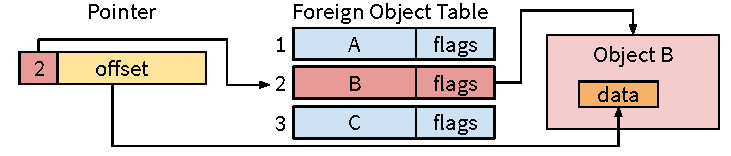
\includegraphics[width=3.5in]{fig/ptrfot}
        \caption{Pointer translation via the FOT\@.
            The pointer and the FOT
            are both contained in the same object (not shown). An FOT entry of $0$ indicates an ``internal''
            pointer.
        }
        \label{fig:fottran}
    \end{figure}

    Instead of \emph{requiring} programmers to refer to objects via IDs only, we allow
    names in FOT entries. These entries may contain a pointer to an
    in-object string table that contains a name.
    %and a function pointer that resolves the name into an
    %object ID.
    Names enable late-binding~\cite{daley:cacm68}, a
    vital aspect of systems, allowing references to objects which change over time, \eg shared library versions.
    Names are passed to a \textit{resolving} function (specified in the FOT entry).
    Allowing a program to specify how its names are resolved
    increases the flexibility of the system beyond supporting \unix paths. \Twizzler
    provides a default name resolver that uses \unix-like paths.% for ease of development of simpler applications.

    The implementation of naming is orthogonal to \Twizzler's design. We
    allow a range of name resolution methods within the system stack
    and allow objects to specify their own name resolution functions for flexibility. For example,
    objects could be organized by both a relational database and a hierarchical namer
    similar to conventional file systems. Non-hierarchical file systems
    are well studied~\cite{gifford:sosp91, ames:mss06, padioleau:usenix03, gopal:osdi99,
        parkerwood:systor14}, but these systems do not easily cooperate atop a single data space.
    Since \Twizzler uses a flat namespace as its ``native'' object naming scheme, it
    enables the required cooperation.

}


\section{Evaluation}

\unedit{
    %rewrite
    We approached these goals two ways: porting existing software (SQLite) and writing new
    software for \Twizzler. The first demonstrates both the generality of the programming environment
    (legacy software can be easily ported) and the potential performance gains to be had even for legacy
    software. The second demonstrates the true power of \Twizzler's programming model and allows us
    to explore the consequences of our design choices fully without being constrained by legacy designs.

    We built three pieces of new software: a hash-table based key-value store (KVS), a red-black tree
    data structure, and a logging daemon. Each had different characteristics and goals, and together
    they demonstrate the flexibility that \Twizzler offers in allowing simple implementation,
    nearly-free access control, and the ability to directly express complex relationships between
    objects.  Using our KVS and red-black tree code, we ported SQLite (a widely used
    SQL implementation) to \Twizzler along with a YCSB~\cite{ycsb,ycsbc} driver (a common benchmark),
    allowing us to explore \Twizzler's model in a larger, existing program that
    would let us study the performance of \Twizzler in a complex system that stores \emph{and
        processes} data. We present the performance of SQLite and our new software, along with microbenchmarks,
    in Section~\ref{sec:res}.
}

\subsection{Case Studies}

\unedit{

    \subsection{Case Study: Key-Value Store}

    %We implemented several applications and data structures to determine the effect of cross-object
    %pointers and \Twizzler's design on programming and system functionality.

    %\subsubsection*{Key-Value Store}
    \label{sec:kv}

    We implemented a multi-threaded hash-table based key-value store (KVS), called \nvkv, to
    study cross-object pointers and our late-binding of access control.
    Our KVS supports insert, lookup, and delete of values by key (both of arbitrary size), and hands
    out direct pointers to persistent data during lookup. During insert, it copies data into a data
    region before indexing the inserted key and value. We built \nvkv in multiple phases to study how
    our system handles changing requirements.

    We built \nvkv in roughly 250 lines of C\@. Handing
    out direct pointers into data was trivial to implement with cross-object pointers, requiring
    only a call to \texttt{ptr\_lea} during lookup. The initial implementation maintains two
    objects, one for data and one for the index.  The complexity typically involved when storing both
    index and data in a single, flat file is not justified in a programming
    model where we can express inter-object relationships directly at
    near-zero cost in complexity or performance. In our case, a pointer from the index object
    to the data object (such as an entry in the hash table) can be written with a single call to
    \texttt{ptr\_store}.
    %to translate the pointer from an offset into the data object into a cross-object
    %pointer for storage in the index. 
    This, combined with the simple requirements for an in-memory \NVM KVS,
    resulted in a small implementation that was nonetheless a
    usable KVS.

    \begin{figure}
        \centering
        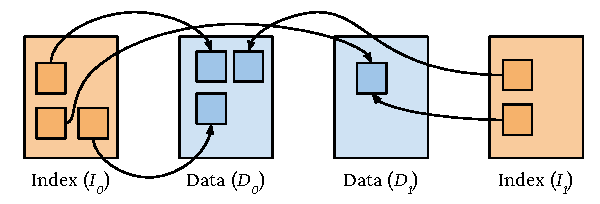
\includegraphics[width=3.5in]{fig/twzkv}
        \caption{Cross-object pointers in \nvkv. The index object contains pointers to keys and values,
            which can reside in any data object. We also support multiple indexes to enable additional
            indexing strategies and access control on discovery. Because \Twizzler provides native support
            for cross-object pointers, this kind of construction is no more complex than keeping all keys
            and data within a single object.}
        \label{fig:twzkv}
    \end{figure}




    \paragraph{Extending Requirements.}

    Next, we added functionality to protect values with access control. We wanted to
    keep handing out direct pointers to data during lookup and to
    keep \nvkv a library (as opposed to a service). Meeting these goals on an
    existing system would be difficult without adding significant
    complexity, such as reimplementing a lot of \Twizzler's pointer framework or implementing manual,
    redundant access control.

    In \Twizzler, implementing access control in \nvkv involved having the index refer to data in
    multiple data objects, assigning those objects different access rights, and allocating from
    those objects depending on desired access rights. We were
    able to implement this while preserving the original code due to the
    transparent nature of \Twizzler's cross-object pointers. Now, when inserting, the application
    indicates the data object into which to copy the data, as shown in Figure~\ref{fig:twzkv}.

    By supporting multiple data objects, \nvkv can leverage the OS's access control,
    minimizing complexity. Unrestricted data can go in $D_0$ (Figure~\ref{fig:twzkv}),
    whereas restricted data can go in $D_1$. Since each object has distinct
    access control, a user can set the objects' access rights, then decide
    where to insert data according to policy. The indexes point to the
    correct locations regardless of the access restrictions of the data objects, and \nvkv still hands
    out direct pointers, but a user that is restricted from accessing data in $D_1$ will not
    be able to dereference the pointer. A further extension is to support secondary indices, as shown in
    Figure~\ref{fig:twzkv}, enabling alternative lookup methods and limiting data discovery
    with index object access control. This extension is easy to implement on \Twizzler.
    %increasing our implementation's complexity only a small amount.

    \paragraph{Comparison to \unix Implementation.} To compare with existing techniques, we built a
    similar KVS using only \unix features (called \unixkv). It also separates index and data, but it
    must manually compute and construct pointers, requiring a significant amount of programmer time to
    get right.
    Supporting multiple data objects was complex in \unixkv, because we had to store and process file
    paths in the index and store references to paths for pointers, increasing overhead and code
    complexity by 36\%---a lot for an implementation with relatively few pointers---just to reimplement
    \Twizzler's support. The extra complexity also included code to manually open, map, and
    grow files, much of which \Twizzler handles internally. Development time was extended by
    bugs that were not present when developing \nvkv, due to the manual pointer processing.  While \nvkv
    gains transparent access control, \unixkv does not due to the lack of
    on-demand object mapping and late-binding of security. Instead, \unixkv needs to know object permissions before
    mapping,
    a restriction that limits the ability to reuse OS access control, something that
    \nvkv could leverage through late-binding on security (\S~\ref{sec:sec})\footnote{\unixkv could trap segmentation faults to do this, but that would be
        application-specific, difficult, and would reimplement \Twizzler functionality.}. Other frameworks like PMDK
    that do not integrate access control and late-binding into their models have similar
    limitations.


    %% TODO RUST SYNTAX
    \subsection{Case Study: Red-Black Tree}
    To evaluate the process of writing persistent, ``pointer-heavy'' data
    structures,
    we implemented a red-black tree in C using normal pointers (\ramrbt)
    in 100 lines of code,
    and evolved it for persistent memory in two ways: manually writing
    base+offset style pointers, as current systems require (\unixrbt),
    and using \Twizzler (\nvrbt).
    Porting existing data structure code to persistent memory
    will be common during the adoption of \NVM, and much of the complexity therein
    comes from dealing with persisting virtual addresses~\cite{virendra:hotstorage17}.

    In developing \unixrbt, we found 83 locations where we had to perform pointer arithmetic for
    converting between persistent and virtual addresses.  Consider an expression such as
    \texttt{root->left->right = foo}. Inserting calls to translate this directly results in
    \texttt{L(L(root)->left)->right = C(foo)}, where \texttt{L} converts to a virtual address and
    \texttt{C} converts back, which is heavily obfuscated and took more development time than writing
    \ramrbt in the first place due to debugging.

    We built \nvrbt like \unixrbt, annotating pointer stores and
    dereferences. However, \unixrbt used an application-specific solution for pointer
    management; if other applications wanted to use the data structures created by \unixrbt, they would
    have to know the implementation details of the pointer system (or share the implementation, thus
    reimplementing much of \Twizzler's library).  Additionally, due to \Twizzler enabling improved
    system-wide support for cross-object pointers, these transformations can be made automatic through
    compiler and linker support.

    Unlike \nvrbt, \unixrbt's tree is limited to a single persistent
    object; a limitation that prevents the tree from growing arbitrarily, does not
    allow it to directly encode references to data outside the tree object, and does
    not gain it the benefits of cross-object data references that were discussed
    above for \nvkv. Adding support for this to \unixrbt would require modifying the
    core data structures to include paths and significantly altering the code,
    increasing its length by at least a factor of 2, whereas \nvrbt gets this
    functionality for free.

    Another advantage of \nvrbt is reduced support code compared to \unixrbt; \unixrbt needed
    code to manage and grow files and mappings, while we implemented \nvrbt as simple data structure code
    with \Twizzler managing that complexity. The additional error handling code and pointer
    validity checks in \unixrbt (handled automatically in \Twizzler) increased development time
    and implementation complexity.


    \subsection{Porting SQLite}

    We ported SQLite to \Twizzler to demonstrate our support for existing software and to evaluate the
    performance of a SQLite backend designed for \Twizzler. We used
    our POSIX support framework, a combination of \texttt{musl} and our library
    \texttt{twix}, to support much of SQLite's POSIX use.
    We took a modified version of SQLite called SQLightning that replaced
    SQLite's storage backend with a memory-mapped KVS called LMDB~\cite{lmdb}.
    We chose this port
    because LMDB is implemented with \texttt{mmap}'d files as the primary access method and hands out
    direct pointers to data as one would expect from an effectively designed \NVM KVS\footnote{These
        are not persistent pointers, however, unlike \Twizzler's.}.
    Since LMDB's SQLightning port already replaces the storage backend
    with calls to
    LMDB, we ported SQLite to \Twizzler by taking our KVS and red-black tree code and implementing
    enough of the LMDB interface for SQLite to run using \Twizzler as a backend.
    Outside of the
    B-tree source file few changes were needed for
    SQLite to run on \Twizzler. We further ported our modified SQLite backend to PMDK to compare
    directly with a commonly used \NVM programming library that supports persistent pointers.

    We also ported a C++ YCSB driver~\cite{ycsbc}, which required porting the C++ standard template
    library (STL). Since we had already ported a standard C library, the C++ STL was easily ported,
    demonstrating the ease of porting software to \Twizzler.
    We have also ported some existing \unix utilities (such as \texttt{bash} and
    \texttt{busybox}), which largely require only recompiling to run on \Twizzler. Of
    course, to gain \emph{all} of the benefits of \Twizzler, programs will be need to be
    written with \NVM in mind (but this is true regardless of the target OS).
    %Our POSIX shim library provides emulated Linux system call support to \texttt{musl},
    %implemented in userspace, such that C programs need only be recompiled.

    Our implementation of the LMDB interface
    corroborated our experience from the KVS case study: much of the complexity in storage interfaces
    and implementations comes from the separation between storage and memory. This has been
    studied before (as we will elucidate in Section~\ref{sec:relwork}), but the advent of \NVM changes the game
    significantly by allowing programmers to think directly via in-memory data structures. The result is
    that interfaces like cursors in a KVS become redundant. We implemented to this interface
    for LMDB, but the functions were largely wrappers around storing a pointer
    to a B-tree node and traversing the tree directly without separate loads and copies. The result was
    an extremely simple implementation (500 LoC) that still met the required interface. Future software
    for \NVM can use \Twizzler's programming model to more effectively write software
    that eschews the need for complexity forced by the two-tier storage hierarchy.

}

\unedit{

    \subsection{Discussion}

    Although these implementations were simple, they represent the applications
    and data structures we expect in a data-centric system. Persistent pointers
    we can directly use in our programming languages make computing over persistent
    data almost transparent, allowing simple implementations that are nevertheless
    easy to evolve as requirements change.
    %The model does not restrict systems
    %applications to shared-memory style interaction; as we saw with \twzlogd,
    %applications can use stream-like, message-passing, and synchronous calling
    %abstractions atop \Twizzler's programming model. These abstractions were
    %similarly easy to build and use, reflecting the simplicity of the data model in
    %\Twizzler.

    Not only does \nvkv have strong support for access control, it enables
    concurrent use of databases via cross-object pointers. Applications can load indexes
    for multiple databases without needing to worry about address space layout and
    without writing complex pointer management code that would be required by an
    implementation using \texttt{mmap}.
    We were able to provide access
    control without a single line of code in \nvkv dedicated to checking or enforcing
    access rights. Instead, we relied on \Twizzler's built-in access control, something not possible with other
    frameworks that do not support late-binding of access rights and do not consider
    security as part of their programming model. \Twizzler thus removes
    the need for applications to enforce and implement their own access control, which
    increases the security of the system by divesting programmers from
    the responsibility of getting the enforcement right.
    Similar functionality for current
    systems would traditionally require separation of the library and application
    into a client-server model, but that additional overhead is unneeded here and
    inappropriate on a persistent memory system.

    Although \nvrbt and \nvkv had different densities of pointer operations, \nvrbt being
    ``pointer-heavy'' and \nvkv being ``pointer-light'', \Twizzler improved the complexity of both
    over manual implementation and improved flexibility over existing persistent
    pointer methods. Using a system-wide standardized approach to
    pointer translations not only enables better compiler and hardware support, but it also improves
    interoperability; because they share a common framework, \nvkv could use the red-black tree code and data with ease, and even interact with
    the SQLite database even though they were written separately without that goal in mind.
    %\emph{because} they share a common framework.
    The position-independence afforded by this model
    enables both composability and concurrency, while also simplifying programming on persistent data to
    a natural expression of data structures.

}

\subsection{Storage Overhead}


\begin{SCfigure}[t]
    \centering
    \includegraphics{genfig/fotoverhead}
    \caption{TODO}
    \label{fig:fotoverhead}
\end{SCfigure}



\subsection{Performance}

\unedit{\label{sec:res}

    %\dab{New experiments we can run!!! Time a linux syscall vs. a twix syscall vs. a twizzler syscall.
    %I have some old data on number of syscalls made by sqlite, but it's from FreeBSD Twizzler. That
    %said, it's unlikely to have changed.}


    Our evaluation's primary focus is on the benefits of the programming model, showing new
    functionality with reduced complexity at an acceptable overhead. Nevertheless, there are many
    cases
    %focused not on performance increase---the
    %benefits of \Twizzler are primarily the programming model---but instead on
    %demonstrating acceptable performance with new functionality and reduced complexity. However, there are many cases
    where we see significant improvement (such as SQLite)
    because the programming model has less overhead, and our pointer design is space
    efficient and fast to translate.
    %In some cases, this is due
    %to fewer system calls, but performance gains also arise elsewhere, as our experiments against
    %SQLightning show.


    We measured the performance of our KVS and red-black tree, performed
    microbenchmarks, and evaluated the \Twizzler port of
    SQLite against Linux (Ubuntu 19.10) instances of SQLite, SQLightning, and our port of SQLite
    to PMDK\@. Tests ran on an
    Intel Xeon Gold 5218 CPU running at 2.30 GHz with 192 GB of DRAM and 128 GB of Intel
    Persistent DIMMs.
    We compiled all tests against the \texttt{musl} C library instead of
    \texttt{glibc} because \Twizzler uses \texttt{musl} to support \unix programs.

    All Linux tests used the NOVA filesystem~\cite{Xu:nova} (a filesystem
    optimized for \NVM) on the NVDIMMs, mounted in DAX mode. This enabled direct access to the
    persistent memory without a page-cache interposing on accesses.
    %The use of persistent memory allows
    %us to account for differences in behavior of the NVDIMMs compared to DRAM.

    \subsection{Microbenchmarks}

    Table~\ref{tbl:res} shows common \Twizzler functions' latencies, including pointer
    translation (loading and storing) and mapping overhead.
    The overhead shown for resolving pointers does not
    include dereferencing the final result, since that is required regardless of how a pointer is
    resolved. The first row shows the latency for resolving pointers to objects the first time.
    \Twizzler makes a further optimization by
    caching the results of translations for a given FOT entry. Each successive
    time that FOT entry is used to resolve a pointer, the result of the original translation is returned
    immediately, improving the latency as shown on the ``cached'' row of Table~\ref{tbl:res}. Note that
    the low latency of these results is expected; the performance critical case of these functions' use
    is repeated calls, and since these operations are simple, they fit within the processor cache.

    \Twizzler translates intra-object pointers by first
    checking if the pointer is internal and, if so, adding the object's base
    address to it---the same operation required for application-specific
    persistent pointers. The expanded programming model offered by \Twizzler
    %and the improved I/O
    %performance
    makes this overhead minor relative to the high costs for persistent data access on
    current systems, which have high-latency for equivalent operations.
    %\textcolor{blue}{While existing frameworks could
    %have similar or slightly faster pointer resolution times, they lack the flexibility our model
    %provides (see Section~\ref{sec:invariant_pointers}) and thus a performance comparison is not as
    %eluciating.}
    %, and the additional work is dwarfed by transfer latencies from memory.

    \begin{table}
        \centering
        \caption{Latency of common \Twizzler operations, including pointer loading and storing, and object
            mapping.
        }
        \begin{minipage}{\linewidth}
            \centering
            \begin{tabular}{c | S[table-format=7.1]@{\,\,\( \pm \)\hspace{-5mm}} S[table-format=0.1]}
                \textbf{Pointer Resolution Action} &
                \multicolumn{2}{c}{\textbf{Average Latency (ns)}} \\
                \hline
                %First-time translation  & 26.9 & 0.1 \\
                %Object already mapped & 5.8 & 0.1      \\
                Uncached FOT translation           & 27.9 & 0.1   \\
                Cached FOT translation             & 3.2  & 0.1   \\
                Intra-object translation           & 0.4  & 0.1   \\
                Inter-object pointer store         & 17.2 & 0.6   \\
                Intra-object pointer store         & 2.3  & 0.1   \\
                Mapping object overhead            & 49.4 & 0.2
            \end{tabular}
        \end{minipage}
        \label{tbl:res}
    \end{table}

    The pointer store operations shown in Table~\ref{tbl:res} measure the latency of the
    \texttt{ptr\_store} operation that is used to construct persistent data references in \Twizzler.
    While these operations are less common than pointer loads, their overhead directly affects
    applications that perform many updates to data structures.
    The most common pointer store operation applications perform is internal (intra-object) pointer stores, in which the
    overhead is minimal. Pointer store operations for external (inter-object) references have slightly
    more overhead, since they need to perform an FOT scan to allow FOT entry reuse.



    We compared our pointer translation to \unix functions.
    Resolving an external pointer with an ID corresponds roughly
    to a call to \texttt{open("id")}, which has a latency of $1036 \pm 15$ ns.
    The comparison is not exact, of course; the pointer resolution
    also maps objects, and the call to \texttt{open} must handle file system
    semantics. However, the direct-access nature of \NVM results in pointer translation
    achieving the same goal as opening a file does today. The pointer operations in \Twizzler accomplish
    much of the same functionality as the heavier-weight I/O system calls on \unix with more utility and
    less overhead.

    %The overhead of system calls is enormous compared to the pointer
    %translation operations of \Twizzler.
    %, although both achieve the result of
    %persistent data access.
    A more direct comparison is object mapping, which has
    low latency compared to \texttt{mmap} ($658.7 \pm 12.7$ ns---a $13.3\times$ speedup) though the two have similar
    functionality. Since mapping occurs entirely
    in userspace, cache pollution is reduced.
    While both \texttt{mmap} and \Twizzler's mapping require
    page-faults to occur before the data is actually mapped,
    this overhead is similar in \Twizzler and \unix, and so is not
    shown.


    %% TODO maybe cut this
    %It is important to keep in context the latency of these operations, many of which 
    %replace relatively heavy \unix operations in functionality in \Twizzler's memory-access
    %model. Most of the equivalent \unix operations require
    %at least one system call, which is untenable for low-latency persistent
    %storage.
    %The mitigations for both Spectre~\cite{spectre} and
    %Meltdown~\cite{meltdown} further motivate reducing system calls, especially with
    %NVM, since they further increase system call latency.


    \subsection{SQLite}

    We ran four variants of SQLite, three on Linux and one on \Twizzler, and compared their performance: ``SQL-Native'' (unmodified SQLite),
    ``SQL-LMDB'' (SQLite using LMDB as the storage backend), ``SQL-PMDK'' (SQLite using
    our red-black tree on PMDK),
    and ``SQL-\Twizzler'' (our port of SQLite running on \Twizzler). SQL-Native was run in \texttt{mmap} mode so that both it
    and SQL-LMDB used \texttt{mmap} to access data.
    We ran each on the same hardware and normalized the results.
    %All were run on the same
    %hardware, and results were normalized.
    %Because the \Twizzler port of SQLite was lacking in full transactional
    %support\footnote{Transaction support is no more difficult in \Twizzler, but as it is not germane, it
    %	was excluded from the study.},
    %we ran experiments with SQLite in read-uncommitted mode. Furthermore, we
    %ran SQL-LMDB and SQL-Native with the database on a ramdisk to remove the overhead of disk
    %I/O and filesystems as much as possible.
    %To get the most performance out of these two variants, we also ran them with
    %asynchronous writes enabled (allowing SQLite to continue after updates without a call to
    %\texttt{fsync} or \texttt{msync}).
    %We normalized results to better show comparisons.
    %rather than raw
    %values.

    Figure~\ref{fig:ycsb} shows the three variants' throughput under standard YCSB
    workloads. The performance improvement of the LMDB and \Twizzler variants over SQL-Native is
    likely due to handing SQLite direct pointers to data. However, in the \Twizzler
    case we get an additional benefit of operating on data structures directly while LMDB has an
    abstraction cost.

    \begin{figure}[t]
        \centering
        \includegraphics[width=4in]{genfig/ycsb}
        \caption{YCSB throughput, normalized (higher is better). \Twizzler outperforms all other
            variants in all tests.}
        \label{fig:ycsb}
    \end{figure}

    Figure~\ref{fig:qlat} shows the latency of queries on a one million row table.
    This is common data processing---loading and then
    examining data in a variety of ways.
    %The transaction overhead is minimal, since the
    %measurements are done on read-only operations.
    We measured the performance
    of calculating the mean and median, sorting rows, finding a specific row,
    building an index, and probing the index. SQL-\Twizzler had similar performance to SQL-LMDB and
    SQL-Native despite comparing its extremely simple storage backend to optimized B-tree
    backends (that benefit from scan operations). As a more direct comparison,
    SQL-\Twizzler significantly out-performed SQL-PMDK in most tests. PMDK's pointer operations are
    more expensive than \Twizzler's, requiring up to two hash table lookups per
    translation~\cite{pmdk-pointers}. Additionally, PMDK's
    pointers are 128~bits, while \Twizzler does not increase pointer size. Increased
    pointer size results in significantly worse cache performance, especially in a pointer-heavy data
    structure like a persistent red-black tree.


    %SQL-\Twizzler out-performed SQLite and SQL-LMDB in
    %every test. The building-index test did not see a dramatic performance improvement, but this largely
    %involved building a volatile in-memory data structure, and thus largely avoided touching persistent memory.

    \begin{figure}[t]
        \centering
        \includegraphics[width=4in]{genfig/qlat}
        \caption{Query latency, normalized (lower is better). \Twizzler maintains a similar level of
            performance with the native and LMDB variants, despite comparing \Twizzler's simplistic
            red-black tree index
            implementation with highly optimized B-trees. \Twizzler also significantly outperforms PMDK
            despite sharing a similar implementation for the index structures.}
        \label{fig:qlat}
    \end{figure}


    \subsection{Key Value Store}
    \label{sec:kvperf}

    We compared \nvkv to \unixkv
    by inserting one
    million distinct key-value pairs, followed by looking up each in-order. The inserted items were 32-bit
    keys and 32-bit values, chosen to reduce the overhead of data copying since we were focusing on
    pointer translation overhead.
    %For similar reasons, we \texttt{memset} the index to zero (to avoid
    %page-fault routines clouding the overhead of pointer translation), and we set the initial hash-table
    %size to avoid expansion (since expansion code is not affected by pointer translations).
    Both were
    compared under two modes, single-data-object and multiple-data-objects. Both KVSes translated
    between virtual and persistent addresses when storing and retrieving data, but for
    multiple-data-objects, we allow for storing the data in an arbitrary object.
    %Finally, we compared to \texttt{clang}'s \texttt{std::unordered\_map} for a baseline, even though
    %\texttt{unordered\_map} does not store data in a separate object and uses virtual addresses instead
    %of persistent pointers.

    Figure~\ref{fig:kvlat} shows the latency of lookup and insert, demonstrating
    that not only is the memory-based index and data object
    structure that can hand out direct data pointers sufficiently low latency to
    take advantage of \NVM,
    %(by our measurement, we are 36$\times$ and 45$\times$
    %faster than Berkeley DB on insert and lookup, respectively),
    but the additional overhead of cross-object
    pointers is minimal.
    %When using a single data object, the overhead is reduced
    %because the system can optimize pointer translations to 2 bitwise operations.
    Compared to \unixkv, \nvkv has minimal overhead in the single-object case, and improves lookup
    performance in the multiple-object case. The minor overhead in other cases comes with improved flexibility,
    simplicity, and access control support (\unixkv does not support access control).
    %Compared to \unixkv, \nvkv improves performance when multiple data objects are supported,
    %has significantly
    %simpler code, and supports access control mechanisms (which \unixkv does not).
    %When using single data objects, \unixkv avoids some of the overhead at the cost of flexiblity.
    %The difference in latency on insert between the KV stores and
    %\texttt{unordered\_map} can be explained by
    %different choices in hashing
    %algorithms,
    %lack of support for persisting the index and data.%, but that the additional overhead was small.
    %, and different
    %optimization levels stemming from code maturity.
    Finally,
    multithreaded access on \nvkv and \unixkv did not improve performance;
    despite the pointer translations, they ran at memory bandwidth (for \NVM).
    %It is important to note that this performance is achieved with stright-forward
    %code using \Twizzler's programming model, while providing the features of a
    %usable KV store. Additionally, access control is provided at little to no
    %additional cost in the implementation---there is no explicit code doing access
    %control checks, instead all access control is handled by the OS
    %during mapping, followed by being handled by the memory system.

    \begin{figure}[t]
        \centering
        \includegraphics[width=4in]{genfig/kvs}
        \caption{Latency of insert and lookup in \nvkv and \unixkv.
            An ``(m)'' indicates
            support for multiple data objects. Both \unixkv and \nvkv have similar latencies.}
        \label{fig:kvlat}
    \end{figure}




    \subsection{Red-Black Tree} We measured the latency of insert and lookup of 1 million 32-bit
    integers on both \unixrbt and \nvrbt. The insert and lookup latency of \nvrbt was $528 \pm 3$ ns
    and $251.8 \pm 0.5$ ns, while insert and lookup latency of \unixrbt was $515 \pm 2$ ns
    and $213 \pm 1$ ns.
    %The lookup overhead of \nvrbt arises because it does not support cross-object trees, while the
    %insert overhead of \unixrbt arises due to the management of the persistent file that is unnecessary
    %in \Twizzler.
    The modest overhead comes with significantly improved flexibility, as \unixrbt does not support
    cross-object trees, and less support code (\unixrbt manually implements mapping and pointer
    translations). Note that even though there is lookup overhead in
    \nvrbt, this overhead did not predict the results of a larger program---the SQL-\Twizzler port used
    this red-black tree, and saw performance benefits over block-based implementations.

    %we still see a performance benefit in a larger application---the SQL-\Twizzler code used
    %this red-black tree internally, and saw performance benefits during queries that were not predicted
    %by this benchmark.
}